\label{chap:introduction}
Introduction goes here...

%---------------------------------------------------------------------
\section{Motivation}
\label{sec:motivation}
Digitalization is ubiquitous these days, no matter if one considers individual
or economical aspects. This trend is accompanied by rising volumes of data and
increasing computationally expensive applications. To cope with related
challenges and in order to serve demands of the market, \enquote{[...] the
computer industry has been driven by an endless quest for more and more
computing power [...]} \cite[p.517 f.]{Tanenbaum.2014}. For decades, increasing
miniaturization along with rising clock speed has been the fundamental approach
in order to advance the performance of processors and digital chips in
general. Unfortunately, there are some considerable limits, wherefore
researchers more and more began to investigate parallelism to continuously
achieve more computing power \cite[p.517 f.]{Tanenbaum.2014}.

%\noindent\rule{\linewidth}{0.4pt}
\vspace{2cm}

Figure example:
\begin{figure}[H]
	\begin{center}
		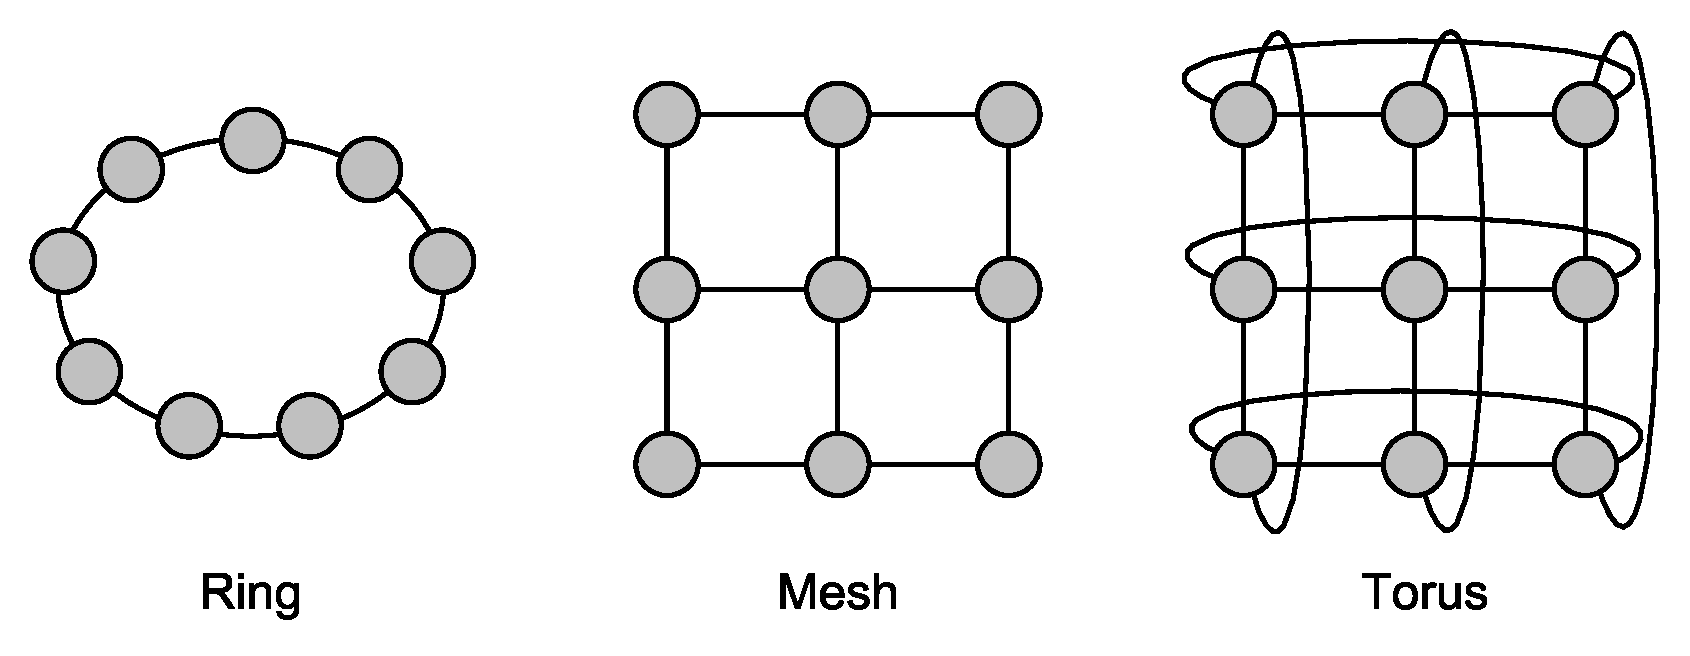
\includegraphics[width=0.7\textwidth]{topologies}
		\caption[Common On-Chip Network Topologies]{Common On-Chip Network Topologies}
		\label{fig:topologies}
	\end{center}
\end{figure}

As illustrated in figure \ref{fig:topologies} ...

\newpage
Table example:
\begin{table}[H]
  \begin{center}
	  \small
	  \begin{tabularx}{0.7\textwidth}{|L!{\vrule width1.2pt}c|c|c|}
		  \hline
		  \textbf{Maximum Speedup} & 8x8 NoC & 16x16 NoC & 32x32 NoC \\  \specialrule{1.2pt}{0pt}{0pt}
		  Group - Size 2 & 9.26 & 54.69 & 113.18 \\ \hline
		  Group - Size 3 & 6.98 & 43.98 & 117.88 \\ \hline
		  Group - Size 4 & 5.7 & 34.56 & 108.85 \\ \hline
	  \end{tabularx}
	  \normalsize
	  \caption[Maximum Speedup Values]{Maximum Speedup Values}
    \label{tab:speedup}
  \end{center}
\end{table}

Compare table \ref{tab:speedup} ...

\vspace{2cm}
Abbreviation example:\\
\acf{MPSoC}\\
\ac{MPSoC}\\

%---------------------------------------------------------------------
% ...
